% include the figures path relative to the master file
\graphicspath{ {./content/method/figures/} }

\section{Segmentation methodology description} 

Optimization methodologies offer a standardized manner to approach segmentation by minimizing an application-driven cost function~\cite{cremers2007review}.
\Cref{fig:method} illustrates a generic representation of the segmentation strategy here adopted to delineate breast tissues or lesions in \ac{us} images. 
The overall segmentation can be seen as a three steps strategy: 
(1) a mapping or encoding of the image into a discrete set of elements $\mathcal{S}$, 
(2) the optimization stage which is formulated as \emph{metric labelling} problem, 
and (3) re-mapping or re-coding of the labels obtained from the previous stage to produce the final delineation. 

\begin{figure}[htpb]
  \centering
  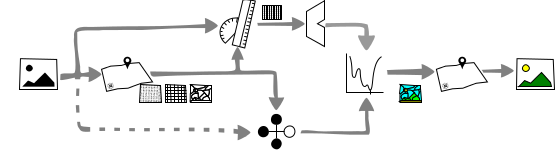
\includegraphics[width=0.9\linewidth]{method}
  \caption{Conceptual block representation of the segmentation methodology}
  \label{fig:method}
\end{figure}

In order to formulate the segmentation like a metric labelling problem, the image is conceived as a discrete set of elements $\mathcal{S}$ that need to be labelled using a label $l$ from the labelling set $\mathcal{L}$ 
(i.e.\, $l \in \{\text{lesion}, \overline{\text{lesion}}\}$ 
or $l \in \{\text{lungs}, \text{fat},\,\cdots\,, \text{lesion}\}$).
Let $\mathcal{W}$ be all the possible labelling configurations of the set $\mathcal{S}$ given $\mathcal{L}$; and, let $U(\cdot)$ be a cost function encoding how good is a labelling configuration $\omega \in \mathcal{W}$ based on the appearance of the elements in $\mathcal{S}$, their inner relation and some designing constrains.
Then, the desired segmentation $\hat{\omega}$ corresponds to the labelling configuration that minimize this cost function, as described in \cref{eq:costMin}.
%minimizing this cost function, $\displaystyle \hat{\omega} = \arg \min_{\substack{\omega}} \,U(\omega)$. 

\begin{equation}
\hat{\omega} = \arg \min_{\substack{\omega}} \,U(\omega)
\label{eq:costmin}
\end{equation}

Selecting the appropriated strategy to minimize the cost function $U(\omega)$ is part of the designing process since depending on the nature of $U(\cdot)$ and $\mathcal{W}$, not all the minimizing strategies are suitable or desirable.

\Cref{eq:labelingeq} shows the details of the cost function which combines two independent cost.
Both costs are shaped by $\mathcal{s}$, evaluated in $\mathcal{W}$ and need to be simultaneously minimized as a whole.
The former term $D_s(\omega_s)$, is referred to as the \emph{data} term, while the latter, $\sum_{r \in \mathcal{N}_{s}} V_{s,r}(\omega_s,\omega_r)$, is indistinctly referred to as the \emph{pairwise} or \emph{smoothing} term.

\begin{equation}
  U(\omega) = \sum_{s\in s} D_s(\omega_s) + \sum_{s}\sum_{r \in \mathcal{N}_{s}} V_{s,r}(\omega_s,\omega_r)
  \label{eq:labelingeq}
\end{equation}

\Cref{fig:methodterms} takes the study case of delineating breast tissues in \ac{us} images, to relate \cref{eq:labelingeq,fig:method}, and offer an interpretation their terms and elements. 

\begin{figure}
    \centering
    \begin{subfigure}[b]{0.19\textwidth}
        \centering
        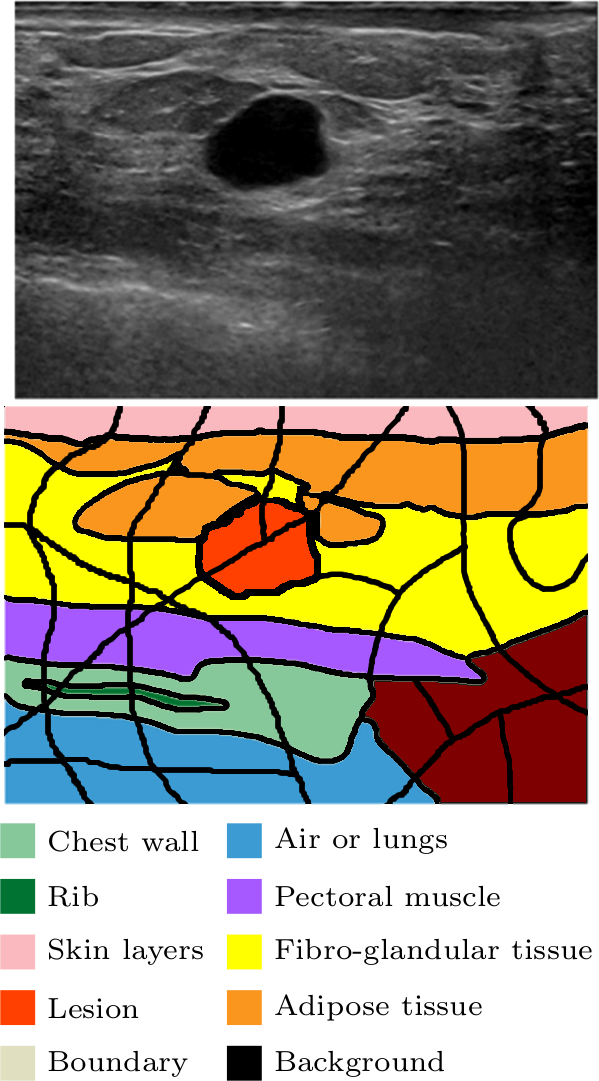
\includegraphics[width=\textwidth]{problem}
        \caption{{\small Problem definition}}    
        \label{fig:methodTerms:problem}
    \end{subfigure}
    \hfill
    \begin{subfigure}[b]{0.39\textwidth}  
        \centering 
        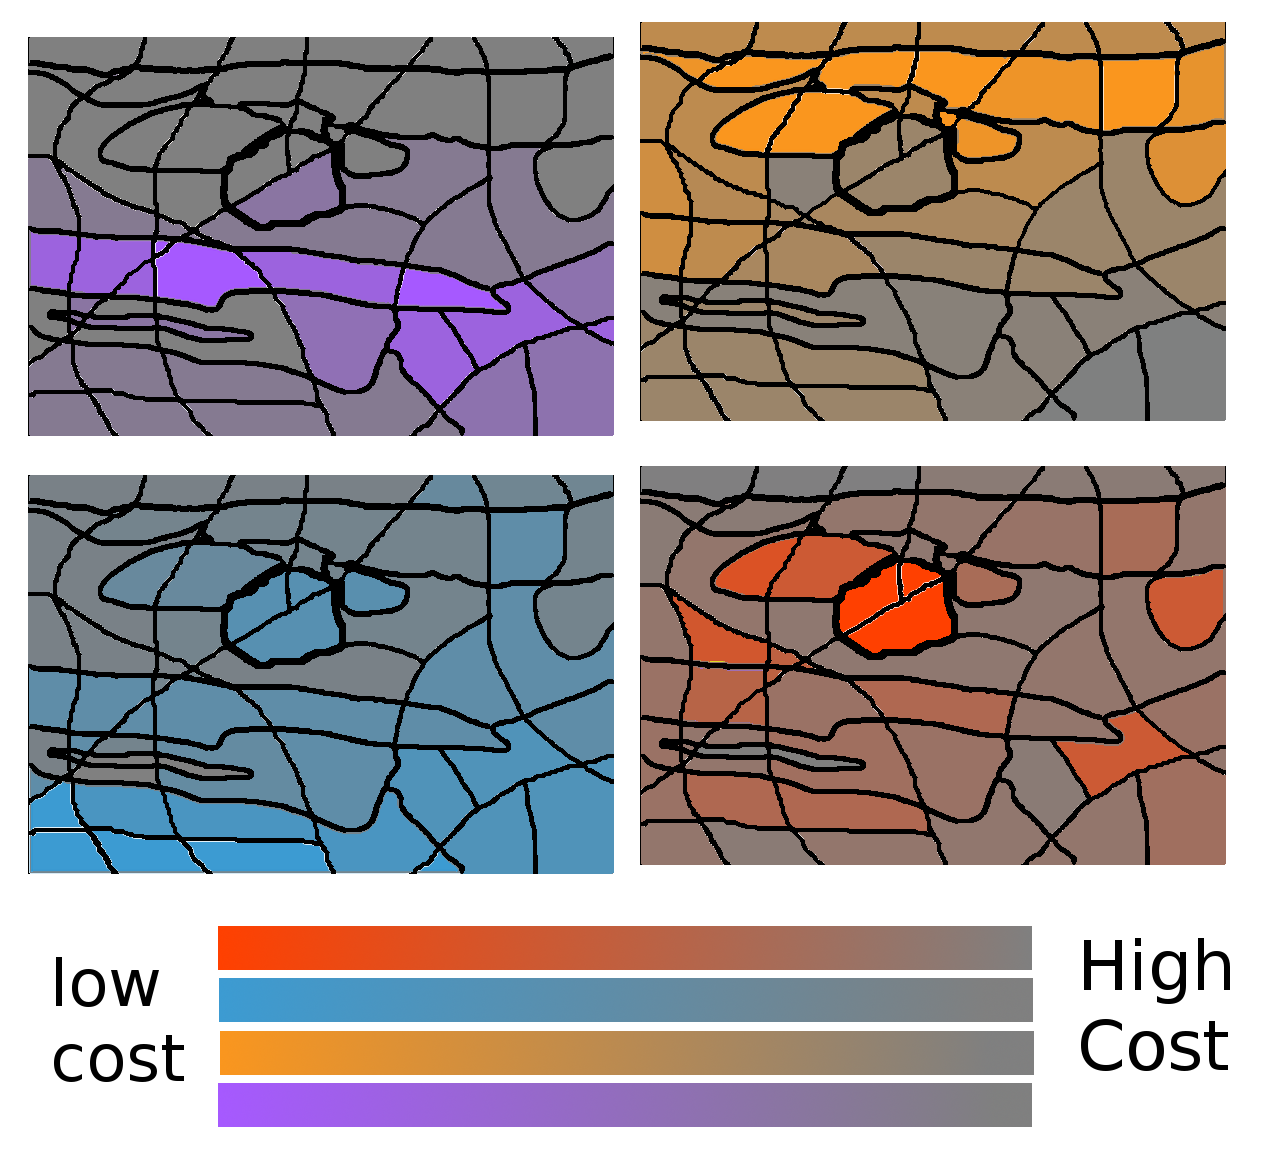
\includegraphics[width=\textwidth]{data}
        \caption[]%
        {{\small Data term}}    
        \label{fig:methodTerms:data}
    \end{subfigure}
    \hfill
    \begin{subfigure}[b]{0.39\textwidth}   
        \centering 
        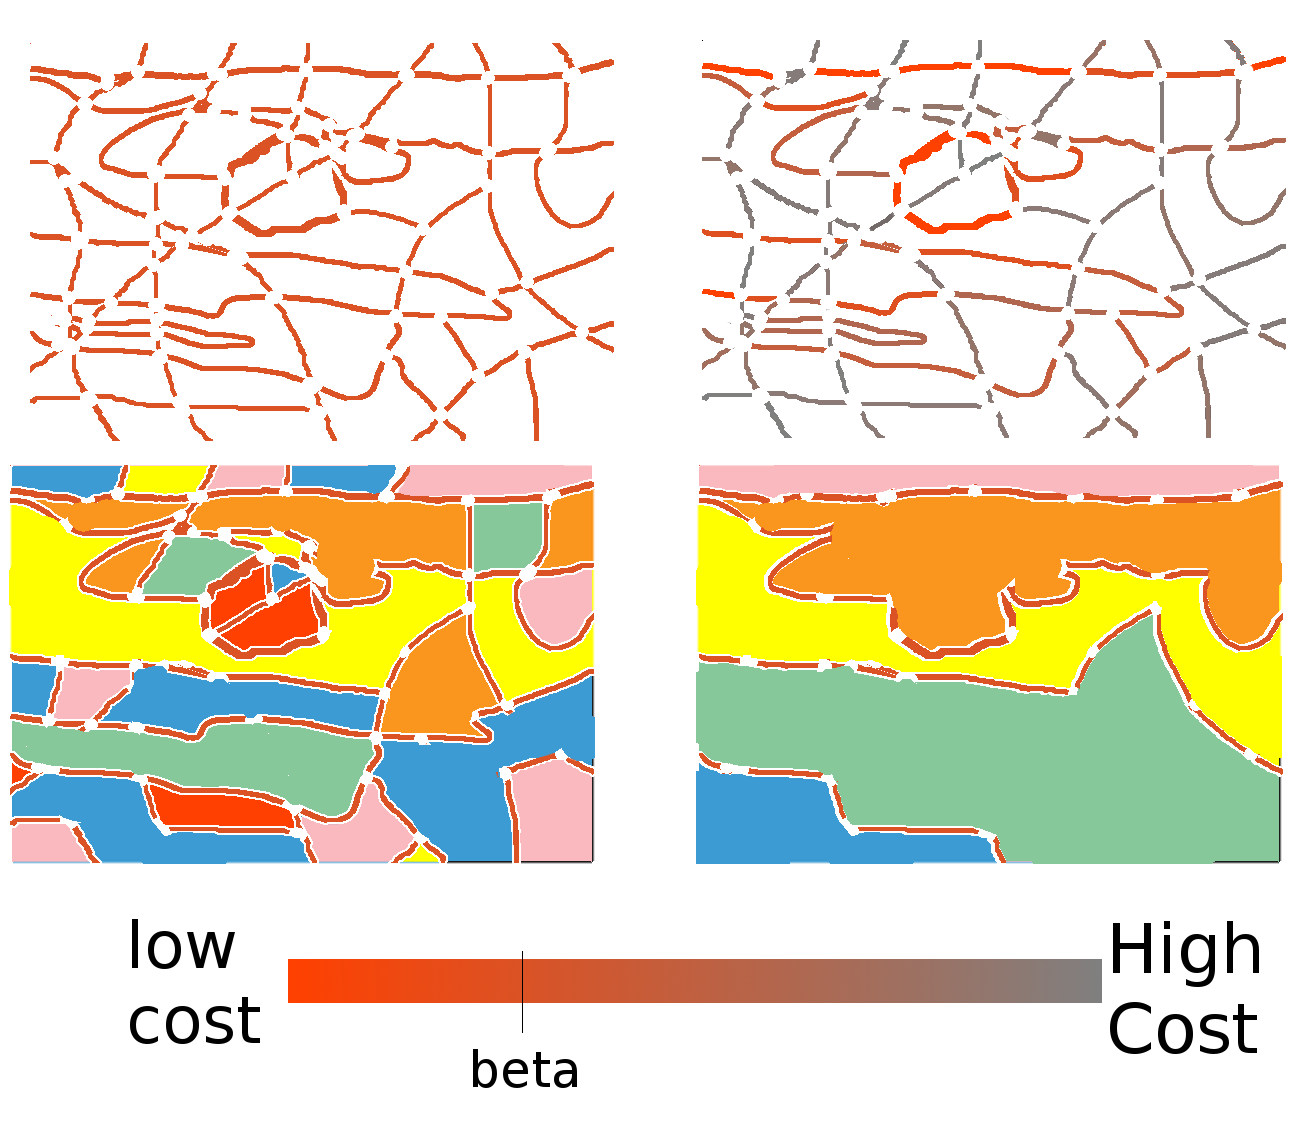
\includegraphics[width=\textwidth]{smooth}
        \caption[]%
        {{\small Pairwise term \emph{for this term the labels should be patterns and the cost be the only color}}}    
        \label{fig:methodTerms:boundary}
    \end{subfigure}
    \caption {\small Methodology terms interpretation} 
    \label{fig:methodterms}
\end{figure}

Despite the fact that $\mathcal{s}$ can be any discrete set representing the image (i.e.\, pixels, overlapping or non overlapping windows, etc.), 
for this application, $\mathcal{s}$ is the super-pixels representation of the image~\cite{achanta2012slic}. 
%The super-pixels can be seen as the output of a over-segmentation process or as a set of pixel collections that are contiguous and coherent with respect to some metric. Either way super-pixels are no overlapped irregular groups of similar connected pixels~\cite{achanta2012slic}.
\Cref{fig:methodTerms:problem} shows a \ac{bus} image example and a its associated super-pixels representation $\mathcal{S}$ coloured according to the image's \ac{gt}.
Bear in mind, that the ultimate goal given an unseen \ac{bus} image is to represent the image as a set of super-pixels and infer the appropriated labelling for each of them.

\subsection{Data term} \label{sec:method:dataTerm}

%Given a label configuration $\omega \in \mathcal{W}$, the data term penalizes the assignation of a particular label to a particular image element or site ($\omega_s = l$) based on the data associated to $s$. 
%In this manner $D_s(\omega_s=l_\cmark) << D_s(\omega_s=l_\xmark)$. 
%To perceive the effect or behaviour of this data term, \cref{fig:methodTerms:data} shows some labelling configurations $\omega^'$ where all the sites share the same label, $\omega' \in \{ \omega_s=l,~\forall s\in\mathcal{S}\}$

Designing $D(\cdot)$ that accomplish the desired behaviour by defining an obscure heuristic, is rather complicated. 
Therefore, an easier and cleaner approach is to take advantage of \ac{ml} techniques. 
The idea is to generate image or data model for each class, based on training samples, and let $D(\cdot)$ be a distance or goodness measure reflecting how likely is for the site $s$ to belong to class $l$.
\Cref{fig:method} shows how this is incorporated to the segmentation framework here proposed.
Each site $s$ is treated as a sample and the features to describe the site are extracted from the original image. 
For the work here reported, a \ac{svm} classifier is used to determine the data model during the training stage and during testing stage $D_s(\omega_s=l)$ corresponds to the distance between the testing sample and the vector supporting the data model associated to $l$. 

Notice that defining $D(\cdot)$ in this manner allows for many designing choices such as: which features to use, how is the class model created: which classifier, which training policy; or, how is defined the relation between the testing sample and the model.
Further discussion regarding the feature choices can be found in \cref{sec:featuers}, whereas other designing choices regarding \ac{ml} are out of the scope for this work.

\subsection{Pairwise or smoothing term} \label{sec:method:mrfTerm}
 
The pairwise term represents the cost of the assignation $\omega_s$ taking into account the labels of its neighbour sites, $\omega_r$, $r \in \mathcal{N}_{s}$. 
This term models a \ac{mrf} or a \ac{crf}.
The typical form of this term, given in \cref{eq:smoothing}, is called homogenization which acts as a regularization factor favouring configurations that have coherent labelling.

\begin{equation}
V_{s,r}(\omega_s,\omega_r) = 
\begin{cases}
    \beta, & \text{if } \omega_s \ne \omega_r\\
    0,              & \text{otherwise}
\end{cases}
\label{eq:smoothing}
\end{equation}

\Cref{fig:methodTerms:boundary} offers a visual interpretation of this cost.
If the resulting segmentation associated to the current labelling configuration $\omega$ has a boundary segment, this boundary brings a penalization $\beta$ to the total cost $U(\omega)$.
In this manner the regularization term can be seen as a post-processing or deionising stage since some sites will flip their labelling if the cost of producing and edge is larger than the cost of adopting the neighbour's label. 

More sophisticated smoothing terms where boundaries contribute have different or variable costs (see \cref{fig:methodTerms:boundary}) are also possible by taking into account not only relations in $\mathcal{S}$ of but also image information (see \cref{fig:method}). 
Further details can be found in \cref{sec:smoothing}.

\subsection{Searching the best labelling configuration}
Once defined $U(\omega)$ so that the cost for a particular labelling configuration $\omega$ can be computed, the problem of finding $\hat{\omega}$ corresponding to the global minimum of the space $\mathcal{W}$ of all possible labelling configurations needs to be faced. 

This problem falls into the category of \textb{NP-hard} problems. 
The dimension of the solution space can be expressed as $||\mathcal{W}|| = ||\mathcal{L}||^{||\mathcal{S}||}$. 
This means that in order to perform an exhaustive search for a toy example of $20$ sites and two possible labels, the cost function needs to be calculated way more than a million times. 
More over, due to limitations in building $U(\cdot)$ such as noise, training policies, etc. there are no guarantees that the global minimum $\hat{\omega}$ corresponds to the true labelling.

Nevertheless, there is a large body of literature proposing methodologies to find suboptimal solutions to the problem trading-off between time of convergence and accuracy of the solution reached.
Szeliski et al.~\cite{szeliski2008comparative} conducted an exhaustive review in terms of solution quality and runtime of the most common energy minimization algorithms used in \ac{cv}, such as \ac{icm}, \ac{sa} or \ac{gc}.

The minimization strategy used for this work is \ac{gc}. 
A technique initially introduced to solve \ac{cv} applications by Boykov et al.~\cite{boykov2001fast} that rapidly become the minimization technique of choice for \ac{cv} problems.
\ac{gc} can only be applied in situations where the pairwise term is designed to favour labelling configurations which are coherent, and to penalize configurations which neighbouring sites do not share labels.
The fact that \ac{gc} can be applied to our cost function, allows to rapidly find a strong local minima guaranteeing that no other minimum with with lower energy can be found~\cite{delong2012fast}. 

\subsection{Similitude with other optimization techniques}
\todo{needs reworking}
It is worth to mention here, that this pairwise term links this segmentation strategy to the family of segmentation methodologies based on optimization using \ac{acm}, such as levelsets.
On its basic form, the family of \ac{acm} segmentation defines some forces to be applied to an initial contour and this contour evolves by minimizing its length while constrained by the forces properly designed for the task in hand.

%
%according to a labelling set 
%
%Which have to be properly labelled and the appropiated label for each element must be infered from a training stage and 
%a discrete set of labels need to properly assigned to another discrete set of elemetns constituting the image.
%
%

%%% Local Variables: 
%%% mode: latex
%%% TeX-master: "../../master.tex"
